\documentclass[11pt,a4paper]{article}
\usepackage[margin=30mm]{geometry}
\usepackage[T1]{fontenc}
\usepackage{lmodern}
\usepackage{amsmath,amssymb,amsthm,mathtools}
\usepackage{microtype}
\usepackage{needspace}
\usepackage{tikz}
\usetikzlibrary{arrows.meta,positioning}
\usepackage[hyphens]{url}
\usepackage[hidelinks]{hyperref}
\hypersetup{pdftitle={A strict inverse-first-power bound for univalent functions},pdfauthor={OpenAI}}
\input{glyphtounicode}
\input{glyphtounicode-cmex}
\pdfgentounicode=1
\pdfglyphtounicode{negationslash}{0338}
\newtheorem{theorem}{Theorem}[section]
\newtheorem{lemma}[theorem]{Lemma}
\newtheorem{proposition}[theorem]{Proposition}
\newtheorem{corollary}[theorem]{Corollary}
\theoremstyle{remark}
\newtheorem{remark}[theorem]{Remark}
\newcommand{\DD}{\mathbb D}
\newcommand{\HH}{\mathbb H}
\newcommand{\C}{\mathbb C}
\newcommand{\R}{\mathbb R}
\newcommand{\E}{\mathbb E}
\newcommand{\KK}{\mathcal K}
\newcommand{\SSS}{\mathcal S}
\newcommand{\ind}{\mathbf 1}
\newcommand{\im}{\operatorname{Im}}
\newcommand{\re}{\operatorname{Re}}
\newcommand{\supp}{\operatorname{supp}}
\newcommand{\rank}{\operatorname{rank}}
\title{A strict inverse-first-power bound for univalent functions}
\author{OpenAI}
\date{September 24, 2026}
\begin{document}
\maketitle
\begin{abstract}
We prove a uniform upper bound for inverse-first-power integral means
of normalized univalent disk maps with exponent strictly below \(1/4\).
Consequently, the bounded universal integral-means spectrum satisfies
\(B_b(-1)<1/4\), disproving Kraetzer's conjectured spectrum at \(p=-1\).
\end{abstract}

\section{Introduction}\label{sec:introduction}

For a univalent function, the derivative can become large or small near
the boundary even when the image domain is bounded. Integral means
measure the rate of this concentration. Their universal spectrum records
the largest possible growth exponent over a class of conformal maps;
it brings questions about derivatives, coefficients, and the geometry
of image boundaries into a common framework.

Let \(\DD=\{z\in\C:|z|<1\}\), and let \(\SSS\) consist of all
injective holomorphic maps \(f:\DD\to\C\) with \(f(0)=0\) and
\(f'(0)=1\). Write \(\SSS_b\) for the subclass of maps with bounded
image. The bound on the image may depend on \(f\), and no boundary
regularity is imposed. For \(p\in\R\) and \(0\le r<1\), define
\begin{align*}
 M_p[f'](r)&=\frac1{2\pi}\int_{-\pi}^{\pi}|f'(re^{i\theta})|^p\,d\theta,\\
 \beta_f(p)&=\limsup_{r\uparrow1}
 \frac{\log M_p[f'](r)}{\log(1/(1-r))},
 &B_b(p)&=\sup_{f\in\SSS_b}\beta_f(p).
\end{align*}
The derivative of a univalent map never vanishes, so all real powers
are defined. The supremum in \(B_b\) is taken after each map's limiting
exponent. Multiplying a map by a nonzero constant leaves that exponent
unchanged, so normalization of the derivative does not change the
bounded-class spectrum.

\subsection{The conjecture and the uniform bound}

Kraetzer's experiments with conformal maps onto bounded domains led
to the prediction
\begin{equation}\label{eq:kraetzer}
 B_b(p)=
 \begin{cases}
 p^2/4,&|p|\le2,\\
 |p|-1,&|p|\ge2.
 \end{cases}
\end{equation}
The quadratic part is stated in his 1996 paper and explicitly
restated in his thesis \cite{Kraetzer,KraetzerThesis}; the full
quadratic--linear formulation also appears in Beliaev's discussion
of numerical spectra \cite{Beliaev}. We prove a strict upper bound
at the negative interior exponent \(p=-1\).

\begin{theorem}[Uniform inverse-first-power bound]\label{thm:main}
There exist constants \(0<\varepsilon<1/4\) and \(C<\infty\) such that
\begin{equation}\label{eq:uniform}
 M_{-1}[f'](r)\le C(1-r)^{-1/4+\varepsilon}
 \qquad\text{for every }f\in\SSS\text{ and every }1/2\le r<1.
\end{equation}
Consequently \(B_b(-1)<1/4\), and Kraetzer's conjectured identity
\eqref{eq:kraetzer} is false.
\end{theorem}

Both constants are independent of the map, including its image size.
The proof gives existence of a positive gap but does not evaluate it
numerically. The conclusion concerns the inverse first power; it does
not settle the proposed value at \(p=1\).

\subsection{Context and the role of strictness}

The distinction between bounded and unrestricted disk maps matters.
Carleson and Jones connected coefficient problems with conformal
dimension \cite{CJ}. Makarov's comparison theorem identifies the
unrestricted spectrum with the maximum of the bounded spectrum and
the Koebe contribution \(3p-1\) \cite[Theorem 5.4]{Makarov}.
In particular, the bounded spectrum in \eqref{eq:kraetzer} should
not be replaced by the unrestricted disk spectrum at positive exponents.
Hedenmalm and Shimorin developed a weighted Bergman-space approach
to bounds for these spectra, keeping this distinction explicit
\cite{HedenmalmShimorin}. Their upper bound at \(p=-1\) for the
unrestricted normalized disk class is \(0.403\)
\cite[Table 1]{HedenmalmShimorin}. Sola subsequently obtained the
bound \(0.388\) by related Bergman-space methods
\cite{Sola}; see also the author's account in
\cite[p.~6]{SolaThesis}. These estimates remain above the
conjectured value \(1/4\); Theorem~\ref{thm:main} establishes a
uniform exponent strictly below it.

Random conformal snowflakes provide another approach. Beliaev and
Smirnov constructed random conformal maps whose averaged spectrum
approaches the universal spectrum at any prescribed exponent, and
related lower bounds to positive integral operators
\cite[Sections 3--4]{BeliaevSmirnov}. Beliaev further investigated
these operators numerically, distinguishing the numerical estimates
from rigorous error control \cite{Beliaev}. The common feature with
the present argument is the use of a law on conformal maps and a
positive operator. Here the operator samples inverse derivatives
through affine changes of base point, and its growth controls an
upper bound uniformly over the entire class \(\SSS\).

The affine-law and saddle-to-maximum construction is also used for
inverse-square means in the companion article
\emph{Brennan's conjecture and sharp inverse-square integral means}
\cite{BrennanMethod}. The two arguments share the compact
normalization of half-plane maps, dyadic sampling, and a comparison
of critical points over a common target. We prove every
inverse-first-power estimate and every transport assertion needed
here; the companion's inverse-square endpoint theorem is not an
input.

The obstacle specific to the present theorem is strictness at the
candidate exponent \(1/4\). A non-strict comparison of saddle and
maximum weights only rules out larger exponents. We retain the exact
operator growth parameter when constructing the probability law.
For almost every target, distinct critical points have distinct
values, so the rank pairing sends each saddle to a strictly higher
maximum. This strict increase forces a vanishing Jacobian in the
remaining equality case. A harmonic lower barrier then excludes
that case. The strict increase can be arbitrarily small from one
pair to another; no common pointwise gain is required.

\subsection{Proof outline}

Section~\ref{sec:operator} transfers disk maps to the compact family
of univalent maps on the upper half-plane \(\HH=\{x+iy:y>0\}\),
normalized by \(F(i)=0\),
\(F'(i)=1\). A positive operator \(L\) samples \(1/|F'|\) at two
affine subscales. The exponential growth rate of \(\|L^n\|\), denoted
by \(2^\beta\), bounds all the disk means in Theorem~\ref{thm:main}.
If \(\beta\ge1/4\), Section~\ref{sec:law} constructs a probability
law whose inverse-derivative weighted rebasings scale exactly as
\(y^{-\beta}\). Differentiating this identity fixes two moments of
the logarithmic derivative.

For a target \(\xi\in\C\), the potential
\(y^{(\beta+2)/3}/|F(x+iy)-\xi|\) turns those moment identities into
a geometric comparison. Section~\ref{sec:escape} proves compactness
of its positive superlevels for almost every map and target.
Section~\ref{sec:pairing} identifies its critical points through a
smooth map \(G_F\), proves the target-generic absence of degeneracies
and ties, and constructs the measurable rank pairing. The nullity of singular
values is the planar instance of Sard's theorem \cite{Sard}; injectivity
supplies the separate exclusion of tied critical values. The planar
index count follows the tangent-turning argument of Hopf \cite{Hopf}.
The moment identities make the expected normalized signed Jacobian
of \(G_F\) positive when \(\beta>1/4\), and zero when \(\beta=1/4\).

Section~\ref{sec:transport} changes variables through \(G_F\) and
compares the paired weights on expanding source rectangles. It also
transfers exceptional-target nullity to the fixed normalized point,
where area-genericity alone would be insufficient.
The comparison forces the expected signed Jacobian to be nonpositive;
strictness of the pairing forces the Jacobian itself to vanish almost
surely in the remaining equality case.
Section~\ref{sec:equality} rules out the vanishing-Jacobian equality
case and converts \(\beta<1/4\) into the uniform estimate.

\section{A compact model and its growth operator}\label{sec:operator}

This section replaces the boundary-growth problem by growth of a
single positive operator on a compact family of normalized maps.

\subsection{Univalence estimates}

We use the classical quarter and derivative-distortion theorems in
exactly the following form \cite[Chapter 2]{Duren}.

\begin{lemma}[Classical univalence estimates]\label{lem:classical}
For every \(f\in\SSS\) and \(|z|=r<1\),
\begin{equation}\label{eq:koebe}
 \frac{1-r}{(1+r)^3}\le |f'(z)|\le
 \frac{1+r}{(1-r)^3},\qquad
 B(0,1/4)\subset f(\DD).
\end{equation}
If \(F\) is univalent on the Euclidean disk \(B(z_0,s)\), then
\begin{equation}\label{eq:local-quarter}
 B\bigl(F(z_0),s|F'(z_0)|/4\bigr)
 \subset F(B(z_0,s)).
\end{equation}
\end{lemma}
\begin{proof}
The first assertions are the quoted classical estimates for normalized
univalent disk maps. Apply the quarter theorem to
\((F(z_0+s\zeta)-F(z_0))/(sF'(z_0))\) to obtain the last assertion.
\end{proof}

Let \(\HH=\{x+iy:y>0\}\), and define
\[
 \KK=\{F:\HH\to\C\text{ univalent}:F(i)=0,\ F'(i)=1\}.
\]
For \(F\in\KK\), set \(Q_F=1/F'\).
With \(m(z)=(z-i)/(z+i)\), the maps of \(\KK\) are exactly
\(F=2i f\circ m\), \(f\in\SSS\).

\begin{lemma}[Compact normalized half-plane family]\label{lem:compact}
The locally uniform topology makes \(\KK\) compact metrizable.
Evaluation of \(F,Q_F\) and all their derivatives is jointly
continuous in \(F,z\), and uniformly bounded on each compact
source set. Moreover, uniformly in \(F\in\KK\),
\begin{equation}\label{eq:strip}
 |Q_F(x+iy)|\le C/y\quad(|x|\le2,\ 0<y\le1),
 \qquad |F(z)|\ge c>0\quad(|m(z)|\ge1/2).
\end{equation}
\end{lemma}
\begin{proof}
Integrating the derivative bound in the disk gives local uniform
boundedness. Montel's theorem gives convergent subsequences.
Limits retain the normalization by convergence of derivatives
and remain injective by Hurwitz's theorem: for a fixed source point,
subtract its value and apply Hurwitz on the punctured domain.
The nonconstant normalization excludes the identically zero
alternative. A countable compact exhaustion metrizes this topology.
Interior holomorphic convergence, together with nonvanishing
derivatives, gives the asserted continuity and bounds.

The identities
\[
 1-|m(z)|^2=\frac{4y}{|z+i|^2},
 \qquad |Q_F(z)|=\frac{|z+i|^2}{4|f'(m(z))|}
\]
and \eqref{eq:koebe} imply the strip estimate.
The image under \(f\) of the disk of radius \(1/2\) contains
\(B(0,1/8)\) by \eqref{eq:local-quarter}. Injectivity gives
the second assertion, with \(c=1/4\) for \(F=2i f\circ m\).
\end{proof}

\subsection{Affine rebasings and dyadic samples}

Identify a point \(z=x+iy\in\HH\) with the affine map
\[
 z\cdot w=x+yw,\qquad z^\#=(-x+i)/y.
\]
This is a group with identity \(i\) and inverse \(z^\#\).
For \(F\in\KK\), define
\[
 (T_zF)(w)=\frac{F(z\cdot w)-F(z)}{yF'(z)}.
\]
Then \(T_zF\in\KK\), and direct substitution gives
\begin{equation}\label{eq:action}
 T_w(T_zF)=T_{z\cdot w}F,\qquad
 Q_{T_zF}(w)=\frac{Q_F(z\cdot w)}{Q_F(z)}.
\end{equation}
On \(C(\KK)\), with its supremum norm, put
\[
 (A_z\Phi)(F)=|Q_F(z)|\,\Phi(T_zF),\qquad
 L=\tfrac12(A_{-1/2+i/2}+A_{1/2+i/2}).
\]
These are bounded positive operators. For each continuous \(\Phi\),
\(A_z\Phi\) is jointly continuous in \(F,z\); rebasings send compact
source sets to compact sets locally in the parameter \(z\).
Equation~\eqref{eq:action} gives \(A_zA_w=A_{z\cdot w}\).
In particular, if
\(v=2^{-n}\) and \(u_j=-1+(2j+1)v\), then
\begin{equation}\label{eq:dyadic}
 L^n=v\sum_{j=0}^{2^n-1}A_{u_j+iv},\qquad
 \|L^n\|=\max_{F\in\KK}(L^n1)(F).
\end{equation}
The abscissae are the sums \(\sum_{\ell=1}^n\pm2^{-\ell}\);
positivity proves the norm identity.
Testing the affine map \(F(z)=z-i\), and using \eqref{eq:strip},
we obtain \(1\le\|L^n\|\le C2^n\).
The same operator will control every map. Submultiplicativity defines
\begin{equation}\label{eq:rho}
 \rho=\lim_{n\to\infty}\|L^n\|^{1/n},
 \qquad \beta=\log_2\rho,\qquad 0\le\beta\le1.
\end{equation}
Indeed, writing \(n=qN+r\), \(0\le r<N\), bounds the upper
root limit by \(\|L^N\|^{1/N}\); take the infimum over \(N\).

\begin{proposition}[From dyadic samples to disk means]\label{prop:disk}
There is a universal constant \(C_0\) such that, for \(f\in\SSS\),
\[
 M_{-1}[f'](r)\le C_0\|L^n\|
 \quad\text{if}\quad 1/2\le r<1,\quad
 v=2^{-n}\le1-r<2v.
\]
Consequently \(B_b(-1)\le\beta\).
\end{proposition}
\begin{proof}
For \(3\pi/4\le\theta\le5\pi/4\), write
\[
 m^{-1}(re^{i\theta})=x+iy,\qquad
 x=\frac{-2r\sin\theta}{d},\quad
 y=\frac{1-r^2}{d},\quad
 d=1-2r\cos\theta+r^2.
\]
Here \(|x|\le1\), \(1/2\le y/v\le4\), and
\[
 \frac{dx}{d\theta}
 =\frac{4r^2-2r(1+r^2)\cos\theta}{d^2}\ge\frac1{16}.
\]
If \(|x-u_j|\le v\), the point
\((x-u_j)/v+i y/v\) lies in a fixed compact rectangle in \(\HH\).
Apply Lemma~\ref{lem:compact} to \(Q_{T_{u_j+iv}F}\) and
\eqref{eq:action} to get
\[
 |Q_F(x+iy)|\le C|Q_F(u_j+iv)|.
\]
For \(F=2i f\circ m\),
\(|f'(re^{i\theta})|^{-1}=4|Q_F(x+iy)|/|x+i(y+1)|^2\).
The denominator is bounded below. Integrating over the cells gives
a bound \(Cv\sum_j|Q_F(u_j+iv)|\le C\|L^n\|\) for this arc.
Four arcs obtained by applying the same argument to
\(e^{-ia}f(e^{ia}\zeta)\) cover the circle.
All constants are independent of \(f\).
Finally \(n/\log(1/(1-r))\to1/\log2\); use \eqref{eq:rho},
take each map's limit superior, and then take the supremum.
\end{proof}


\section{A weighted affine law}\label{sec:law}

We next turn excessive operator growth into an exact scaling identity
for a probability law. For the remainder of the argument suppose,
toward a contradiction, that
\begin{equation}\label{eq:contrary}
 \beta\ge1/4.
\end{equation}
All laws below are constructed at this fixed exponent.

\begin{proposition}[Exact-parameter affine law]\label{prop:law}
Assume \(\beta=\log_2\rho\ge1/4\), where \(\rho\) is defined in
\eqref{eq:rho}. There is a Borel probability \(P\) on \(\KK\) such that, writing
\(\E\) for expectation under \(P\),
\begin{equation}\label{eq:law}
 \E\bigl[|Q_F(x+iy)|\,\Phi(T_{x+iy}F)\bigr]
 =y^{-\beta}\E\Phi(F)
\end{equation}
for every \(x+iy\in\HH\) and every nonnegative Borel test
\(\Phi:\KK\to[0,\infty]\).
\end{proposition}
\begin{proof}
We use the representation of positive functionals on continuous
functions of a compact metric space by Borel measures
\cite[Theorem 7.2]{Folland}.
Compactness of probabilities follows by taking a diagonal limit on
a countable dense family of continuous tests and applying this
representation theorem.

\emph{The operator eigenmeasure.} First construct a probability \(\mu\) with \(\mu L=\rho\mu\),
where measures act on the left as integration functionals.
For \(\tau>\rho\), the series
\[
 R_\tau=\sum_{n\ge0}\tau^{-n}L^n,\qquad
 g_\tau=R_\tau1,\qquad M_\tau=\max g_\tau
\]
converges in operator norm. Since
\[
 Lg_\tau=\tau(g_\tau-1)
 \le\tau(1-1/M_\tau)g_\tau,\qquad 1\le g_\tau\le M_\tau,
\]
positivity gives
\(\|L^n\|\le M_\tau[\tau(1-1/M_\tau)]^n\).
Thus \(\rho\le\tau(1-1/M_\tau)\), so
\(M_\tau\ge\tau/(\tau-\rho)\to\infty\).
At a maximizer \(F_\tau\) of \(g_\tau\), the functional
\(\mu_\tau=\delta_{F_\tau}R_\tau/M_\tau\) is a probability and
\[
 \mu_\tau L=\tau\mu_\tau-\frac{\tau}{M_\tau}\delta_{F_\tau}.
\]
A weak limit as \(\tau\downarrow\rho\) gives the required \(\mu\).

\emph{Horizontal and scale averages.} The composition law gives
\(A_{u+iv}A_{2+i}=A_{u+2v+iv}\): right translation by \(2\)
shifts the grid in \eqref{eq:dyadic} by one cell of width \(2v\).
Using \(\mu=\rho^{-n}\mu L^n\), all but the two endpoint terms cancel:
\[
 \mu A_{2+i}-\mu
 =\rho^{-n}v\bigl(\mu A_{1+v+iv}-\mu A_{-1+v+iv}\bigr).
\]
The norm of this difference is at most \(2C\rho^{-n}\) by
\eqref{eq:strip}, and tends to zero because \(\beta>0\).
Therefore \(\mu A_{2+i}=\mu\).
It follows that \(t\mapsto\mu A_{t+ih}\) has period two for every
fixed \(h>0\).

Define
\(\bar\mu=\tfrac12\int_0^2\mu A_{x+i}\,dx\) on continuous tests.
Periodicity gives \(\bar\mu A_{s+i}=\bar\mu\) for all \(s\in\R\).
Moreover,
\[
 \rho\bar\mu
 =\tfrac12\int_0^2\mu L A_{x+i}\,dx
 =\tfrac12\int_{-1/2}^{3/2}\mu A_{t+i/2}\,dt
 =\bar\mu A_{i/2}.
\]
The middle equality uses \(t=-1/2+x/2\) and \(t=1/2+x/2\)
for the two summands of \(L\); the last uses period two.
Consequently \(h^\beta\bar\mu A_{ih}\) is multiplicatively
two-periodic in \(h>0\).
Each of these functionals is horizontally invariant on the right,
because \(A_{ih}A_{s+i}=A_{hs+i}A_{ih}\).
The functional
\[
 \nu=\int_1^2 h^\beta\bar\mu A_{ih}\,\frac{dh}{h}
\]
has finite, strictly positive mass by compact-family continuity.
Periodicity and the substitution \(u=hy\) give
\(\nu A_{iy}=y^{-\beta}\nu\). Horizontal invariance persists,
so normalization of \(\nu\) gives \eqref{eq:law} for continuous tests.
For each fixed \(x+iy\), the two sides define finite Borel measures
(one is a weighted pushforward). Equality on continuous tests makes
them equal as measures, proving the assertion for all nonnegative
Borel tests.
\end{proof}

The law now supplies the differential moments needed for the signed
Jacobian comparison. For \(z=x+iy\), define
\begin{equation}\label{eq:qk}
 q_F(z)=iy\,\frac{Q_F'(z)}{Q_F(z)}
       =-iy\,\frac{F''(z)}{F'(z)}=a_F(z)+ib_F(z),
 \qquad k=\frac{\beta+2}{3}.
\end{equation}
Thus \(3(k-1)=\beta-1\) and \(3/4\le k\le1\).
Equation~\eqref{eq:action} implies
\(q_{T_zF}(w)=q_F(z\cdot w)\).

\begin{lemma}[Logarithmic-derivative moments]\label{lem:moments}
The law satisfies
\begin{equation}\label{eq:moments}
 \E a_F(i)=-\beta,\qquad
 \E|q_F(i)|^2=\beta(\beta+1).
\end{equation}
\end{lemma}
\begin{proof}
The constant test in \eqref{eq:law} gives
\(\E|Q_F(x+iy)|=y^{-\beta}\).
Since \(\log|Q_F|\) is harmonic,
\[
 \partial_y|Q_F|=\frac{|Q_F|a_F}{y},\qquad
 \Delta|Q_F|=|Q_F|\left|\frac{Q_F'}{Q_F}\right|^2.
\]
Differentiate at \(i\), where \(Q_F(i)=1\).
Lemma~\ref{lem:compact} and local nonvanishing give the uniform
smoothness bounds needed to differentiate under expectation.
\end{proof}

\section{Compact superlevels for almost every target}\label{sec:escape}

The affine law must next control escape in the source half-plane.
Our objective is compactness of positive superlevels, which will make
the subsequent critical-point counts finite above each positive value.
For \(F\in\KK\) and \(\xi\in\C\), put
\[
 V_\xi^F(x+iy)=\frac{y^k}{|F(x+iy)-\xi|},
\]
with value \(+\infty\) at the possible pole.
The choice \(3k=\beta+2\) lets a submean estimate for \(|1/F|^3\)
convert the weighted area tail below into decay of \(V_0^F\) at
source infinity.
We write \(dA\) for planar Lebesgue area.

\begin{proposition}[Compact positive superlevels]\label{prop:compact-levels}
For \(P\)-almost every \(F\), and then for area-almost every
\(\xi\in\C\), every closed positive superlevel
\(\{V_\xi^F\ge\delta\}\), \(\delta>0\), is compact in \(\HH\).
\end{proposition}

We prove this by controlling infinity and then the real boundary.
The order of these two controls is useful: the first supplies
a horizontal preimage-length bound for the second. That bound is
uniform in the height, with the map and compact target set fixed.

\begin{lemma}[The weighted area tail]\label{lem:area-tail}
Writing \(S_0=\{z\in\HH:|m(z)|\ge1/2\}\), almost every \(F\) satisfies
\begin{equation}\label{eq:area-tail}
 I(F):=\int_{S_0}y^\beta|F(z)|^{-3}\,dA(z)<\infty.
\end{equation}
\end{lemma}
\begin{proof}
For fixed \(z\ne i\), apply \eqref{eq:law} to
\(\Phi(F)=|F(z^\#)|^{-3}\).
The identity
\((T_zF)(z^\#)=-F(z)Q_F(z)/y\) gives
\[
 \E\bigl[|F'(z)|^2|F(z)|^{-3}\bigr]
 =y^{-\beta-3}\E|F(z^\#)|^{-3}.
\]
The integral of the left side over \(S_0\) is uniformly finite:
by injectivity and \eqref{eq:strip}, it is bounded by
\(\int_{|\omega|\ge c}|\omega|^{-3}\,dA(\omega)\).
The involution \(z\mapsto z^\#\) preserves \(|m(z)|\), inverts
the height, and has absolute Jacobian \(y^{-3}\).
Changing variables on the right leaves exactly the weight \(y^\beta\).
Tonelli proves finite expectation of \(I\), hence the assertion.
\end{proof}

\begin{lemma}[Escape at infinity and horizontal length]\label{lem:infinity}
If \(I(F)<\infty\), then
\begin{equation}\label{eq:infinity}
 \frac{y^k}{|F(x+iy)|}\longrightarrow0
 \qquad\text{as } |x|+y\longrightarrow\infty.
\end{equation}
For every compact target set \(K\), its preimage restricted to
\(y\ge\epsilon>0\) is compact, its whole preimage has bounded height,
and
\begin{equation}\label{eq:horizontal}
 \sup_{s>0}\int_\R\ind_K(F(x+is))\,dx<\infty.
\end{equation}
\end{lemma}
\begin{proof}
If \(w=x'+iy'\in B(z,y/2)\), then \(y/2\le y'\le3y/2\) and
\(|x|+y\le |x'|+3y'\).
Thus these disks escape every bounded \(|x'|+y'\) region as
their centers do. The complement of \(S_0\) is bounded, so
the disks are eventually contained in \(S_0\) and avoid the zero of \(F\).
Submean for \(|1/F|^3\), together with \(3k=\beta+2\), gives
\[
 \left(\frac{y^k}{|F(z)|}\right)^3
 \le C_\beta\int_{B(z,y/2)}
      (\im w)^\beta|F(w)|^{-3}\,dA(w).
\]
The right side tends to zero as a tail of \eqref{eq:area-tail}.
For \(|F(z)|\) bounded and \(y\ge\epsilon\), this excludes source
infinity, proving strip compactness. It also excludes unbounded
heights in the whole preimage of \(K\).

Choose a nonnegative smooth compactly supported \(\psi\ge\ind_K\)
and put \(H(y)=\int_\R\psi(F(x+iy))\,dx\).
For fixed \(s>0\), the support in \(y\ge s/2\) is compact by the
strip assertion. Hence differentiation and integration by parts give
\begin{align*}
 H(s)&=\int_s^\infty(y-s)H''(y)\,dy\\
 &=\int_{y>s}(y-s)|F'(z)|^2(\Delta\psi)(F(z))\,dA(z).
\end{align*}
Here the integral of \(\partial_{xx}(\psi\circ F)\) is zero and
\(\Delta(\psi\circ F)=|F'|^2(\Delta\psi)\circ F\).
If \(Y_\psi\) bounds the preimage heights of \(\supp\psi\), the
absolute value is at most
\[
 Y_\psi\int_\HH |F'(z)|^2|(\Delta\psi)(F(z))|\,dA(z)
 \le Y_\psi\int_\C|\Delta\psi|\,dA.
\]
The last inequality uses injectivity, and the bound is independent
of \(s\). This proves \eqref{eq:horizontal}.
\end{proof}

\begin{proof}[Proof of Proposition~\ref{prop:compact-levels}]
Fix \(F\) satisfying Lemma~\ref{lem:area-tail}. The preceding
lemma controls source infinity. It remains to control approach to the
real boundary, uniformly in the horizontal coordinate for almost every
target.
For omitted targets, meaning \(\xi\notin F(\HH)\), restrict to
\(|\xi|\le R\) and fix \(\delta>0\).
At scale \(h=2^{-\ell}\), \(\ell\ge0\), partition the line into
cells \([jh,(j+1)h)\). Mark a cell if some point \(z=x+iy\)
with \(x\) in that cell and \(h\le y\le2h\) satisfies
\(|F(z)-\xi|\le y^k/\delta\) for at least one such omitted target.
At a witness, \eqref{eq:local-quarter} on \(B(z,y)\) gives
\(y|F'(z)|\le4|F(z)-\xi|\).
For every \(x'\) in the same cell, the rebased point
\((x'-x)/y+i h/y\) belongs to the compact rectangle
\([-1,1]+i[1/2,1]\). Lemma~\ref{lem:compact} applied to \(T_zF\)
therefore gives
\begin{equation}\label{eq:cell-cover}
 |F(x'+ih)-\xi|\le C_\delta h^k.
\end{equation}
This bound holds for every witness and its target.

Each marked cell's entire segment at height \(h\) is mapped into
\(\{|\omega|\le R+C_\delta\}\).
Equation~\eqref{eq:horizontal} thus bounds the number of marked
cells by \(C/h\).
Disks of radius \(C_\delta h^k\) centered at their midpoint images
cover all targets witnessed at this scale, and have summed area
\(O(h^{2k-1})\).
The sum over dyadic scales is finite because \(k>1/2\).
The limsup of these measurable covering unions has area zero.
Taking integer \(R>0\) and \(\delta=1/n\), \(n\ge1\), shows that
for almost every omitted target,
\[
 \sup_x V_\xi^F(x+iy)\longrightarrow0\qquad(y\downarrow0).
\]
Indeed a failure at arbitrarily small heights gives witnesses
in infinitely many dyadic bands for one such threshold.

If \(\xi\in F(\HH)\), a small closed disk about \(\xi\) contained
in \(F(\HH)\) has compact inverse image under the homeomorphism
onto the image. Below its minimum preimage height,
\(|F(z)-\xi|\) is uniformly positive, giving the same limit.
At heights bounded below, \eqref{eq:infinity} gives
\(|F(z)|\to\infty\) and \(V_\xi^F(z)\to0\) at source infinity.
Finally \(\{V_\xi^F\ge\delta\}\) is relatively closed, since it is
\(\{|F(z)-\xi|\le y^k/\delta\}\), also at a pole.
The two escape exclusions prove its compactness.
\end{proof}

\section{Critical points and strict pairing}\label{sec:pairing}

For \(P\)-almost every map and area-almost every target, our next goal is to pair
each saddle of the potential with a higher non-pole local maximum.
Compact superlevels and nondegeneracy will supply finite critical-point
counts above positive levels.

\subsection{The critical map}

Define the smooth real map and its normalized signed Jacobian by
\begin{equation}\label{eq:G}
 G_F(z)=F(z)-\frac{iyF'(z)}k,\qquad
 J_F(z)=\frac{\det DG_F(z)}{|F'(z)|^2}.
\end{equation}
Its real derivative columns are
\((F'/k)(k+q_F)\) and \((iF'/k)(k-1+q_F)\).
Consequently
\begin{equation}\label{eq:Jacobian}
 k^2J_F=k(k-1)+(2k-1)a_F+|q_F|^2,\qquad
 k^2\E J_F(i)=\frac{(4\beta-1)(\beta+2)}9.
\end{equation}
The second identity uses \eqref{eq:moments} and \(k=(\beta+2)/3\).

Off the possible pole, write \(\ell=\log V_\xi^F\) and
\(r_0=F'/(F-\xi)\). Then
\[
 \Delta\ell=-k/y^2,\qquad
 (\ell_x,\ell_y)=(-\re r_0,\ k/y+\im r_0).
\]
Critical points are therefore exactly the preimages \(G_F(z)=\xi\).
A pole is not such a preimage. At a critical point,
\begin{equation}\label{eq:critical-value}
 V_\xi^F(z)=k y^{k-1}|Q_F(z)|,\qquad
 r_0'=\frac{k(k+q_F)}{y^2}.
\end{equation}
Since \(3(k-1)=\beta-1\), cubing the critical value produces
\(k^3y^{\beta-1}|Q_F(z)|^3\). This is the weight, up to the constant
\(k^3\), that the target change of variables in
Section~\ref{sec:transport} will assign to each critical point.
Direct differentiation yields
\begin{equation}\label{eq:hessian}
 \operatorname{Hess}\ell
 =\frac{k}{y^2}
 \begin{pmatrix}-(k+a_F)&b_F\\b_F&k-1+a_F\end{pmatrix},
 \qquad
 \det\operatorname{Hess}\ell=-\frac{k^4}{y^4}J_F.
\end{equation}
Its trace is negative. Thus \(J_F>0\) gives a nondegenerate saddle,
and \(J_F<0\) a nondegenerate local maximum. We call the latter
a \emph{finite maximum}, excluding a pole.

\subsection{Good targets}

Let \(\mathcal G\subset\KK\times\C\) be the set of pairs
\((F,\xi)\) for which all positive closed superlevels
of \(V_\xi^F\) are compact, \(\xi\) is a regular value of \(G_F\),
and distinct preimages under \(G_F\) have distinct \(V_\xi^F\)-values.
We call these pairs \emph{good}.

\begin{lemma}[Generic targets and Borel goodness]\label{lem:good}
Goodness is Borel in \((F,\xi)\). For \(P\)-almost every \(F\),
area-almost every \(\xi\) is good.
\end{lemma}
\begin{proof}
The superlevel assertion is Proposition~\ref{prop:compact-levels}.
For any fixed \(F\), singular values of \(G_F\) have area zero.
This is the plane case of Sard's theorem \cite[Theorem 4.1]{Sard}.
Here is the elementary estimate needed for this smooth plane map.
On a compact source box, cover singular points by grid squares
of side \(h\). Linearize at one singular point of each square.
Bounded second derivatives put its image in an \(O(h^2)\)-neighborhood
of a segment of length \(O(h)\). Its area is \(O(h^3)\).
There are \(O(h^{-2})\) squares, giving total area tending to zero.
Exhaust the source by compact boxes.

Cover the nonsingular locus by countably many inverse-function
charts. On an overlap where two branches \(z_1(\xi),z_2(\xi)\)
are distinct, the target differential of their critical log values is
\[
 d_\xi\bigl[\log V_\xi^F(z_j(\xi))\bigr](v)
 =\re\frac{v}{F(z_j(\xi))-\xi}.
\]
The source derivative vanishes by criticality.
The two linear functionals differ by injectivity of \(F\).
Hence the difference of log values has nonzero differential, and
its zero set is locally a smooth curve. Countably many chart pairs
give an area-null tie set.

For measurability, use
\(C_m=\{|x|\le m,\ 1/m\le y\le m\}\).
For every integer \(n\ge1\), require the open set
\(\{V_\xi^F>1/n\}=\{|F(z)-\xi|<ny^k\}\) to lie in some \(C_m\).
Failure of a given containment is detected at rational-coordinate
points outside the closed box. This is a Borel test.
It is equivalent to compactness of all closed positive superlevels:
for a closed level choose a strictly smaller reciprocal-integer
threshold and use relative closedness.

Failures of regularity or absence of ties are witnessed by one or
two points in a common \(C_m\). For a tied pair impose separation
at least \(1/n\), and test the values by the continuous expression
in \eqref{eq:critical-value}. Equality conditions and this separation
condition have closed parameter projections because the source
boxes are compact. Countably many \(m,n\) prove the other Borel tests.
\end{proof}

If \(t\in\HH\), \(Y=\im t\), and
\(\eta=(\xi-F(t))/(YF'(t))\), direct calculation gives
\begin{align}
 G_{T_tF}(w)&=\frac{G_F(t\cdot w)-F(t)}{YF'(t)},&
 J_{T_tF}(w)&=J_F(t\cdot w),\label{eq:G-action}\\
 V_\eta^{T_tF}(w)&=Y^{1-k}|F'(t)|\,V_\xi^F(t\cdot w).
 &&\label{eq:V-action}
\end{align}
Thus goodness corresponds in both directions under rebasing.

\subsection{The superlevel count}

\begin{lemma}[The superlevel index count]\label{lem:count}
For a good pair and \(h>0\),
\begin{equation}\label{eq:count}
 \#\{z:\ z\text{ is a finite maximum},\ V_\xi^F(z)\ge h\}
 \ \ge\
 \#\{z:\ z\text{ is a saddle},\ V_\xi^F(z)\ge h\}.
\end{equation}
Both counts are finite.
\end{lemma}
\begin{proof}
The fiber \(G_F^{-1}(\xi)\) is closed and discrete, and the closed
positive superlevel is compact. This proves finiteness. There can
be no accumulation at a pole either, because a pole is not on the fiber.

First count in \(U=\{V_\xi^F>\lambda\}\) for a positive regular
level \(\lambda\). We will show that each component is bounded by
one simple closed curve and has total gradient index one, giving
\begin{equation}\label{eq:index-count}
 \#\text{components}
 =\#\text{finite maxima}-\#\text{saddles}+\#\text{poles}
 \quad\text{in }U.
\end{equation}
The boundary of \(U\) is the compact smooth one-manifold
\(\{V_\xi^F=\lambda\}\), away from any pole.
It is a finite disjoint union of smooth simple closed curves.
For detail, the components are open in this compact manifold, so
there are finitely many. Each component is one orbit of the smooth
unit tangent field obtained by rotating \(\nabla\ell/|\nabla\ell|\).
The orbits are complete and open. A nonperiodic single orbit would
be a bijective local homeomorphism from \(\R\) to the compact
component, which is impossible. Its least period gives a simple
closed curve.

The bounded Jordan interior of each curve has closure in \(\HH\):
the region below the curve's minimum height lies in the unbounded
complement. Everywhere inside, \(V_\xi^F>\lambda\). Otherwise
\(\ell\) would have an interior minimum, contrary to
\(\Delta\ell=-k/y^2<0\). If a pole is present, remove a sufficiently
small neighborhood where \(\ell\) is large before taking this minimum.
Thus curves cannot be nested, and their interiors are exactly the
components of \(U\). Indeed each component meets the level boundary,
has its superlevel side locally inside one of the curves, and cannot
leave that interior without crossing the level.

On each positively oriented curve, \(\nabla\ell\) points inward
and has winding one. We recall the tangent-turning argument
of Hopf \cite[Section 2]{Hopf}.
Parametrize a simple regular curve by \(\gamma:[0,1]\to\C\),
with matching endpoint derivatives, starting at a leftmost point.
The positive tangent initially points down. The unit secant direction
from \(\gamma(s)\) to \(\gamma(t)\), \(0\le s\le t\le1\),
extends continuously to the diagonal by the tangent, and to
\((0,1)\) by the negative initial tangent.
Lift its angle continuously on this triangle.
On \((0,t)\) it lies in the closed right semicircle and changes
angle by \(\pi\). On \((s,1)\) it is the negative of the direction
at \((0,s)\), giving another \(\pi\).
The diagonal therefore records tangent winding one, unchanged for
the inward normal.

Remove disjoint small disks about the finitely many critical points
and possible pole in each component. Stokes applied to the closed
angle form
\[
 \frac{X_1\,dX_2-X_2\,dX_1}{|X|^2},\qquad X=\nabla\ell,
\]
shows that the sum of interior indices is one.
At a nondegenerate critical point the index is the sign of the
Hessian determinant, hence \(+1\) for a maximum and \(-1\) for
a saddle. At the pole \(z_0\),
\(\ell=-\log|z-z_0|+\text{a smooth function}\), giving index \(+1\).
Summing over components proves \eqref{eq:index-count}.
There is at most one pole; if present it belongs to a component.
Thus the finite-maximum count is at least the saddle count.
This also covers the empty superlevel.

Finally choose a regular \(\lambda<h\) with no critical value
in \([\lambda,h)\). Such a choice is possible by finiteness
above \(h/2\). The counts in \(U\) are then the counts in
\eqref{eq:count}.
\end{proof}

\subsection{Measurable rank pairing}

The count gives an intrinsic assignment: match the two decreasing
lists by rank. Measurability requires a separate argument, because
we will integrate the assignment over maps and source points. General
countable-section uniformization is supplied by the Lusin--Novikov
theory; see \cite[4F.6 and 4F.17]{Moschovakis}. In the present
setting, local inverse branches give an elementary enumeration, while
intrinsic ranks ensure equivariance.

\begin{proposition}[Strict measurable rank pairing]\label{prop:pair}
On the Borel domain
\[
 \mathcal D=\{(F,z):J_F(z)>0,\ (F,G_F(z))\in\mathcal G\}
\]
there is a Borel assignment \(R_F(z)\) to a finite maximum over
the same target, injective on each target fiber, such that
\begin{equation}\label{eq:strict-value}
 V_{G_F(z)}^F(R_F(z))>V_{G_F(z)}^F(z).
\end{equation}
It is equivariant:
\[
 R_F(t\cdot w)=t\cdot R_{T_tF}(w)
\]
on the corresponding domains.
\end{proposition}
\begin{proof}
On each good fiber order saddles by decreasing critical value,
and separately order finite maxima the same way.
Each point has finitely many predecessors. A nonempty list has a
first point: choose any one point and inspect the finite nonempty
set at or above its value. Repeating gives integer ranks for all points.
Lemma~\ref{lem:count} supplies at least as many maxima as saddles
at or above each saddle's value. Pair the saddle of rank \(j\)
with the maximum of rank \(j\).
No ties are allowed, so the paired value is strictly larger,
as illustrated in Figure~\ref{fig:ranks}.
Different ranks give different partners. Equation~\eqref{eq:V-action}
preserves ranks, proving equivariance.

We prove the measurability assertion directly using the nonsingularity
of each root.
The nonsingular solution graph \(G_F(z)=\xi,\ J_F(z)\ne0\)
has countably many continuous local root branches \(b_j(F,\xi)\),
defined on open parameter sets.
To obtain a branch near \((F_0,\xi_0,z_0)\), set
\(M=DG_{F_0}(z_0)\). On a sufficiently small closed source ball,
\[
 w\longmapsto w-M^{-1}(G_F(w)-\xi)
\]
has Lipschitz constant at most \(1/2\) for all nearby parameters.
Shrinking the parameter neighborhood makes the displacement of
the center less than half the radius. The map is a contraction
of the ball into itself, with a unique interior nonsingular root.
Compactness and uniqueness imply continuous dependence on the
parameters. These branches form relatively open graph patches;
second countability of \(\KK\times\C\times\HH\) gives a countable cover.

At each parameter activate branch \(j\) only when it is defined
and its value differs from every earlier defined branch value.
This Borel test enumerates each root once.
The signs of \(J\), critical values \eqref{eq:critical-value},
and comparisons of such values are Borel. On good fibers,
counting active predecessors of the same sign gives Borel integer
ranks. Selecting the unique active negative-sign branch of the
same rank as a given active positive-sign branch is therefore Borel.
Substitute \(\xi=G_F(z)\) to obtain the claimed assignment.
\end{proof}

\begin{figure}[tbp]
\centering
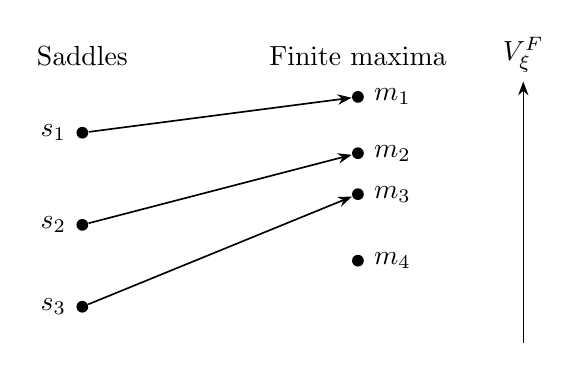
\begin{tikzpicture}[x=1cm,y=.65cm,
 point/.style={circle,fill,inner sep=1.5pt},
 >={Stealth[length=5pt]}]
 \node at (0,5.6) {Saddles};
 \node at (3.5,5.6) {Finite maxima};
 \foreach \j/\sy/\my in {1/4.1/4.8,2/2.3/3.7,3/.7/2.9}{
   \node[point,label=left:{$s_{\j}$}] (s\j) at (0,\sy) {};
   \node[point,label=right:{$m_{\j}$}] (m\j) at (3.5,\my) {};
   \draw[->,semithick] (s\j) -- (m\j);
 }
 \node[point,label=right:{$m_4$}] at (3.5,1.6) {};
 \draw[->] (5.6,0) -- (5.6,5.1) node[above] {$V_\xi^F$};
\end{tikzpicture}
\caption{Schematic rank ordering on one good fiber \(G_F^{-1}(\xi)\).
Both lists are ordered by decreasing critical value, and equal ranks
are paired. Distinct critical values put each paired maximum strictly
above its saddle. Heights represent values rather than spatial
positions; the displayed counts and gaps are illustrative.}
\label{fig:ranks}
\end{figure}


\section{Strict weighted transport}\label{sec:transport}

The pairing will imply \(\E J_F(i)\le0\), with equality only if
\(J_F(i)=0\) almost surely. Comparing this conclusion with
Equation~\eqref{eq:Jacobian} will reduce the contradiction to a
rigidity argument.

Put \(J_{F,\pm}=\max(\pm J_F,0)\) and
\(\omega_F(z)=y^{\beta-1}|Q_F(z)|\).
For any fixed \(F\) and nonnegative Borel \(h\), local change of variables
gives
\begin{equation}\label{eq:area-formula}
 \int_\HH h(z)\omega_F(z)J_{F,\pm}(z)\,dA(z)
 =
 \int_\C\!
 \sum_{\substack{G_F(z)=\xi\\ \pm J_F(z)>0}}
 h(z)y^{\beta-1}|Q_F(z)|^3\,dA(\xi).
\end{equation}
Indeed cover the indicated sign locus by countably many local
diffeomorphism charts, disjointify into Borel pieces, and use absolute
Jacobian \(|J_F||F'|^2\). No global properness of \(G_F\) is required.
At a preimage, \eqref{eq:critical-value} and \(3(k-1)=\beta-1\) give
\begin{equation}\label{eq:target-weight}
 y^{\beta-1}|Q_F(z)|^3=(V_\xi^F(z)/k)^3.
\end{equation}

\begin{lemma}[Goodness at the normalized point]\label{lem:base-good}
The positive-Jacobian mass at the base point is supported on good fibers:
\begin{equation}\label{eq:base-good}
 \E\bigl[J_{F,+}(i)
       \ind_{\{(F,G_F(i))\text{ not good}\}}\bigr]=0.
\end{equation}
\end{lemma}
\begin{proof}
For almost every \(F\), bad targets have area zero by
Lemma~\ref{lem:good}. Formula~\eqref{eq:area-formula} therefore gives
\[
 \int_{\{|x|\le1,\ 1\le y\le2\}}
 \omega_F(z)J_{F,+}(z)
 \ind_{\{(F,G_F(z))\text{ not good}\}}\,dA(z)=0.
\]
The product of \(J_{F,+}\) and the indicator equals its base-point
version for \(T_zF\), by \eqref{eq:G-action}--\eqref{eq:V-action}.
Take expectations and apply \eqref{eq:law} and Tonelli.
The spatial density is \(dx\,dy/y\); its integral on this box is
\(2\log2>0\). This proves \eqref{eq:base-good}.
\end{proof}

The weighted assertion is essential: \(G_F(i)=-i/k\) for every \(F\),
so area-genericity alone says nothing about this fixed target.
We need only the weighted conclusion, not almost-sure goodness
at the base point without the Jacobian factor.

\Needspace{10\baselineskip}
\begin{proposition}[Strict weighted transport]\label{prop:strict-transport}
Assume \(\beta\ge1/4\), let \(P\) be the law of
Proposition~\ref{prop:law}, and set \(k=(\beta+2)/3\).
Then \(\E J_F(i)\le0\).
Equality is possible only if \(J_F(i)=0\) almost surely.
\end{proposition}
\begin{proof}
For \(N\ge1\), restrict the pairing domain \(\mathcal D\) to
\(\mathcal D_N\) by requiring, for \(z'=R_F(z)=x'+iy'\),
\[
 1/N\le y'/y\le N,\qquad |x'-x|\le Ny.
\]
These Borel sets increase to \(\mathcal D\), and their indicators
at \((F,z)\) equal their indicators at \((T_zF,i)\).
Define the equivariant Borel ratio
\[
 c_F(z)=
 \left(\frac{V_{G_F(z)}^F(R_F(z))}{V_{G_F(z)}^F(z)}\right)^3>1
 \quad\text{on }\mathcal D,
\]
and set it to zero elsewhere.
For \(S>0\), \(Y>1\), use the boxes
\[
 B=\{|x|\le S,\ 1\le y\le Y\},\qquad
 B'=\{|x|\le S+NY,\ 1/N\le y\le NY\}.
\]
Every included saddle in \(B\) has its partner in \(B'\).
On the target side of \eqref{eq:area-formula}, multiplication
by \(c_F\) makes its weight exactly the partner's weight
by \eqref{eq:target-weight}. Fiberwise injectivity of the pairing
therefore proves, for every \(F\),
\[
 \int_B\omega_FJ_{F,+}c_F\ind_{\mathcal D_N}(F,z)\,dA(z)
 \le\int_{B'}\omega_FJ_{F,-}\,dA(z).
\]
Take expectations and apply \eqref{eq:law} to the equivariant
nonnegative tests. The resulting inequality is
\begin{align*}
 2S\log Y\,
 \E[J_{F,+}(i)c_F(i)\ind_{\mathcal D_N}(F,i)]
 \le
 2(S+NY)(\log Y+2\log N)\,\E J_{F,-}(i).
\end{align*}
Here \(J_F(i)\) is bounded by compact-family continuity, so
the right side is finite. At fixed \(N\), first let \(S\to\infty\),
then \(Y\to\infty\). Finally let \(N\to\infty\) by monotone
convergence. This gives
\[
 A:=\E[J_{F,+}(i)c_F(i)\ind_{\mathcal D}(F,i)]
 \le d:=\E J_{F,-}(i).
\]
Lemma~\ref{lem:base-good} gives
\(b:=\E J_{F,+}(i)=\E[J_{F,+}(i)\ind_{\mathcal D}(F,i)]\).
Thus \(b\le A\le d\), proving \(\E J_F(i)\le0\).
If equality holds, then \(b=d\) and
\[
 0\le\E[J_{F,+}(i)(c_F(i)-1)\ind_{\mathcal D}(F,i)]
 =A-b\le0.
\]
The integrand is strictly positive wherever \(J_{F,+}(i)>0\)
on \(\mathcal D\). Equation~\eqref{eq:base-good} removes positive
mass outside this domain, so \(b=0\), and hence \(d=0\).
No uniform positive gap in \(c_F-1\) is needed.
\end{proof}

\section{The harmonic equality barrier and the uniform gap}\label{sec:equality}

The moment identity and strict transport can coexist at
\(\beta\ge1/4\) only in the equality case \(\beta=1/4\).
We first rule out its deterministic consequence, an identically
vanishing Jacobian, and then transfer that obstruction back to the law.

\begin{lemma}[The harmonic equality barrier]\label{lem:no-zero-J}
For \(k=3/4\), no \(F\in\KK\) has \(J_F\equiv0\).
\end{lemma}
\begin{proof}
By \eqref{eq:Jacobian}, such a map would satisfy
\[
 |q_F(z)+1/4|^2=1/4.
\]
Therefore \(|q_F(z)|\ge1/4\) and
\(|F''(z)/F'(z)|\ge1/(4y)\).
The pre-Schwarzian has no zeros, so
\(u=\log|F''/F'|\) is harmonic and \(u\ge-\log4-\log y\).
For \(0<\epsilon<1/2\), the harmonic function
\[
 b_\epsilon(x,y)=-\log4+
 \log(1/\epsilon)\cos(\pi x/2)
 \frac{\sinh(\pi(1-y)/2)}{\sinh(\pi/2)}
\]
lies below \(u\) on the boundary of
\([-1,1]\times[\epsilon,1]\).
On its sides and top the added term is zero; on its bottom
the cosine-sinh factor is between zero and one.
The minimum principle gives \(u\ge b_\epsilon\) inside.
At \(i/2\), the coefficient of \(\log(1/\epsilon)\) is fixed
and positive, contradicting finiteness as \(\epsilon\downarrow0\).
\end{proof}

\begin{proof}[Proof of Theorem~\ref{thm:main}]
Under \eqref{eq:contrary}, Equation~\eqref{eq:Jacobian} and
Proposition~\ref{prop:strict-transport} force
\(\beta=1/4\), \(k=3/4\), and \(J_F(i)=0\) almost surely.
Apply \eqref{eq:law} to the test \(|J_F(i)|\).
By \eqref{eq:G-action} and the strictly positive weight
\(|Q_F(z)|\), \(J_F(z)=0\) almost surely at every fixed \(z\).
A countable dense set and continuity give \(J_F\equiv0\)
for almost every \(F\), contradicting Lemma~\ref{lem:no-zero-J}.
Thus the single exponent in \eqref{eq:rho} satisfies \(\beta<1/4\).

Choose \(b\) with \(\beta<b<1/4\).
The root limit in \eqref{eq:rho} supplies a constant \(C_b\)
such that \(\|L^n\|\le C_b2^{bn}\) for all \(n\).
Proposition~\ref{prop:disk}, with \(2^{-n}\le1-r<2^{1-n}\),
then gives \(M_{-1}[f'](r)\le C(1-r)^{-b}\), uniformly in
\(f\in\SSS\). Taking \(\varepsilon=1/4-b\) proves
\eqref{eq:uniform} and the stated disproof.
\end{proof}



\bibliographystyle{alphaurl}
\bibliography{references/references}
\end{document}
